%%%%%%%%%%%%%%%%%%%%%%%%%%%%%%%%%%%%%%%%%%%%%%%%%%%%%%%%%%%%%%%%%
%
% Project     : Bachelorarbeit
% Title       : Machbarkeitsanalyse für eine ressourcenorientierte Schnittstelle zur Verarbeitung grundlegender Probleme der Informatik
% File        : fazit.tex Rev. 01
% Date        : 01.03.2015
% Author      : Raffael Santschi
%
%%%%%%%%%%%%%%%%%%%%%%%%%%%%%%%%%%%%%%%%%%%%%%%%%%%%%%%%%%%%%%%%%


\chapter{Schlussfolgerungen}\label{chap.Schlussfolgerungen}
In der Schlussfolgerung wird kurz auf die Verwendung des Produktes, das Fazit des Verfassers und den Ausblick eingegangen.

\section{Verwendung}\label{fazit_verwendung}
Während der Projektzeit konnte der Spielplan des Auffahrtsturniers des Turnverein Grafstals validiert werden. Dieser Spielplan wird von Hand erstellt und immer wieder unterlaufen 
kleine Patzer, was bei einer Planung von etwa 110 Spielen und Schiedsrichtern, welche Coaches für bis zu drei Teams sind, nicht verwunderlich ist. Diese Aufgabe hat zum einen die Schnittstelle 
getestet, hat jedoch auch dem Verein geholfen, da auch dieses Jahr zwei kleine Fehler auftauchten. Der Turnverein hat sich bereits sehr für die vollautomatisierte Lösung interessiert.

\section{Fazit}\label{fazit}

Das Erstellen eines Konzept einer solchen Schnittstelle stellte sich als sehr spannend heraus. Die Recherche und die Analyse der Probleme mit hoher Laufzeitkomplexität war sehr fesselnd und es 
bestand die Gefahr sich darin zu verlieren. Das Gebiet der theoretischen Informatik ist extrem weitreichend und die Probleme können beliebig komplex werden. Es war schnell klar, dass es schwierig 
sein wird, eine generische Lösung für die Probleme zu finden. Das Konzept mit dem pre- und post-Aktionen ist eine elegante Lösung und bietet sehr viel Flexibilität. Der Ablauf einer Berechnung 
konnte generisch gehalten werden und somit ist die Machbarkeitsstudie als erfolgreich zu betrachten.

Die Auswahl der Probleme hat sich als facettenreich herausgestellt und das Auswahlverfahren hat sich bewährt. Es ist spannend, dass die beiden Probleme aus dem Bereich `Netzwerk Design' 
viele Ähnlichkeiten aufzeigen, jedoch mit komplett anderen Algorithmen gelöst werden. Die beiden Planungsprobleme sind sich sehr ähnlich und könnten ziemlich sicher mit einem generischen 
Algorithmus gelöst werden. Der grösste Unterschied liegt darin, dass bei einem Spielplan zwei Mannschaften gleichzeitig auf einem Platz sind und bei einem 
Stundenplan jeweils nur eine Klasse. Der Code der Schnittstelle konnte für die Planungsprobleme auch viel generisch gehalten werden als für die beiden aus dem Bereich `Netzwerk Design'.

Der Entscheid, eine dokumentorientierte Datenbank zu verwenden, war ideal. Die Flexibilität der Datenbank kam dem Projekt sehr zu gute und es wurde keine Funktion vermisst. Spring Boot ist für 
einen Prototyp ideal, da es schon sehr viel mitbringt. Dies kann jedoch auch zu Problemen führen, da die Versionen von den Libraries nicht selber verwaltet werden können. 

Ich bin mit dem Konzept und dem entstanden Prototyp sehr zufrieden und freue mich nun auf die Planung der nächsten Schritte. Mit Spannung erwarte ich die ersten realen Kunden, welche diese 
Schnittstelle verwenden und bin gespannt, wohin sich diese entwickelt. Ich bin mir bewusst, dass die Schnittstelle noch keine Produktionsreife hat. Es benötigt jedoch nicht mehr viel, bis die ersten 
Turnierpläne vollautomatisch erstellt werden können.

\section{Ausblick}\label{fazit_ausblick}

Das Konzept ist nun ausgearbeitet, jetzt wird eine automatisierte Lösung angestrebt. Als nächstes wird die Integration von zwei Teilprojekten, welche sich um die Entwicklung eines 
Verarbeitungssystem mit einer Cloud Lösung und um die Ansteuerung eines generischen Planungsalgorithmus handeln, geplant. Danach wird es weiteren Entwicklungsaufwand geben, da ein 
Webseite für die Eingabe für Kleinkunden angedacht ist. Da die Endlösung schlussendlich dem Nutzer eine ungefähre Berechnungszeit angeben möchte, wird eine Berechnungskomponente 
benötigt. Diese Komponente wird wahrscheinlich mittels Heuristiken und alten Resultaten eine Zeitextrapolation bestimmt. Die Grundsteine für diese Berechnung sind mit dem vorgestellten Konzept 
bereits gelegt. Die Zwischenresultate und Endresultate enthalten einen Zeitstempel und dadurch kann berechnet werden, wie lange die Berechnung zu einem gewissen Resultat gedauert hat. In 
\autoref{fig:ausblick} ist das Konzept des übergeordneten Projekts dargestellt, von welchem Teile des User API und der Data Controller in diesem Projekt behandelt wurden.

\begin{figure}[h]
\centering
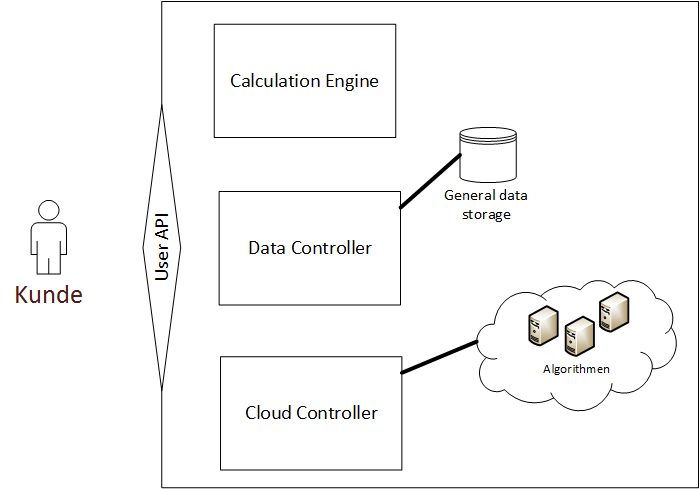
\includegraphics[scale=0.8]{images/visio/ausblick.png}
\caption[Konzept des übergeordneten Projekts]{Konzept des übergeordneten Projekts \selfmade{}}
\label{fig:ausblick}
\end{figure}